\documentclass[11pt]{article}
\usepackage{amsmath}
% use UTF8 encoding
\usepackage[utf8]{inputenc}
% use KoTeX package for Korean
\usepackage{kotex}

\usepackage{hyperref}

\usepackage{graphicx}

\hypersetup{
    colorlinks=true,   
    urlcolor=red,
}

\title{머신러닝}

\author{Minwoo Jung}

\begin{document}

\maketitle

\section{CNN}

\subsection{전체구조}

\indent \\합성곱 신경망(CNN)은 이미지 및 음성을 인식할 수 있는 가장 기본 딥러닝 기법이다. 인접하는 계층의 모든 뉴런과 결합되어 있는 상태를 완전연결(Fully connected)이라고 정의하며, 완전히 연결된 계층을 Affine 계층이라고 부른다. Affine 변환은 기하학에서 행렬의 곱을 부르는 이름이다. 
	\begin{figure}[h!]
		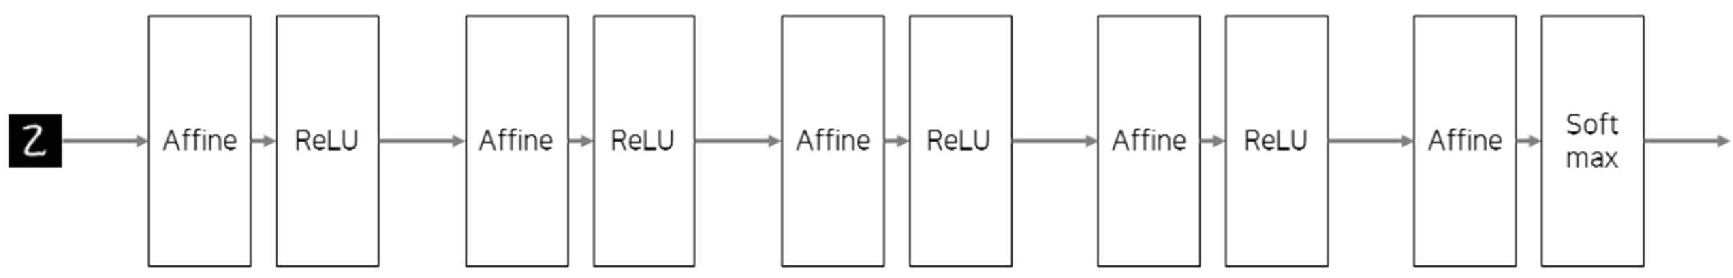
\includegraphics[width=1\columnwidth]{../Figure/Figure_1.pdf}
        \label{Fig.1}
	\end{figure}
\indent \\CNN이 도입되면서 합성곱계층(Convolutional layer)과 풀링계층(Poolling layer)이 새롭게 등장한다.  
    \begin{figure}[h!]
		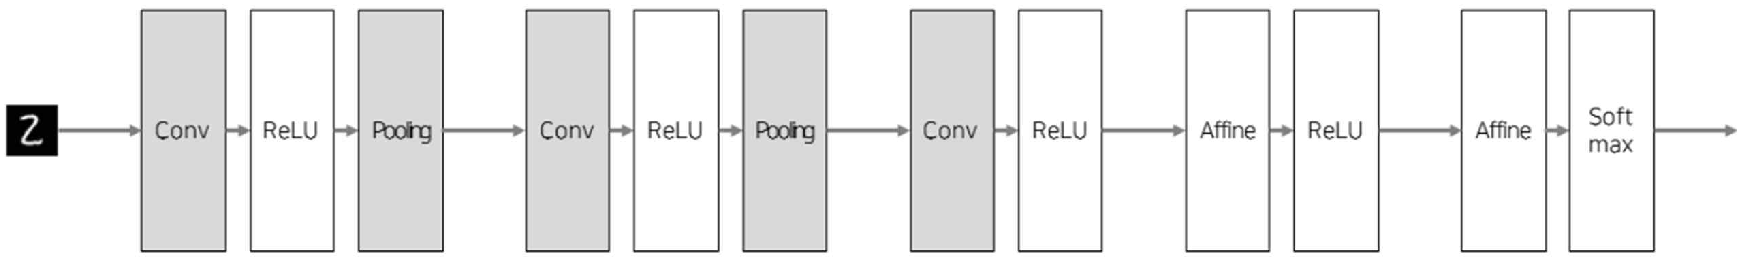
\includegraphics[width=1\columnwidth]{../Figure/Figure_2.pdf}
        \label{Fig.2}
	\end{figure}	
\indent \\'Affine-ReLU' 연결이 CNN 계층으로 바뀌면서 'Conv-ReLU-(Pooling)'으로 바뀌었다.

\subsection{합성곱계층}

\subsubsection{완전연결 계층의 문제점}
\indent \\완전연결계층에서는 인접하는 계층의 뉴런이 모두 연결되고 출력의 수는 임의로 정할 수 있다. 하지만, 완전연결의 문제점은 데이터 형상이 무시된다. 예를 들면, 이미지는 3차원 데이터(가로, 세로, 색상)이지만 완전연결계층에 입력할 때는 1차원 데이터로 바꿔줘야한다. 합성곱 계층은 형상을 유지한다. 이미지도 3차원 데이터로 입력받아서 형상을 가진 데이터로 제대로 이해할 수 있다. CNN에서 합성곱 계층의 입출력 데이터를 특징맵이라 하고, 입력 데이터를 입력 특징맵, 출력 데이터를 출력 특징맵이라고  한다. 
\subsubsection{합성곱 연산}
합성곱 연산은 이미지 처리에서 말하는 필터 연산이다. 입력데이터에 필터를 적용한다. 필터 윈도우를 일정 간격으로 이동하면서 입력데이터에 적용한다. 입력과 필터에 대응하는 원소끼리 곱한 후 그 총합을 구한다. 문헌에 따라 필터를 커널이라고 칭하기도 한다. 필터의 윈도우는 그림\ref{Fig.3} 회색 3*3 부분을 가리킵니다. 
\begin{figure}[h!]
    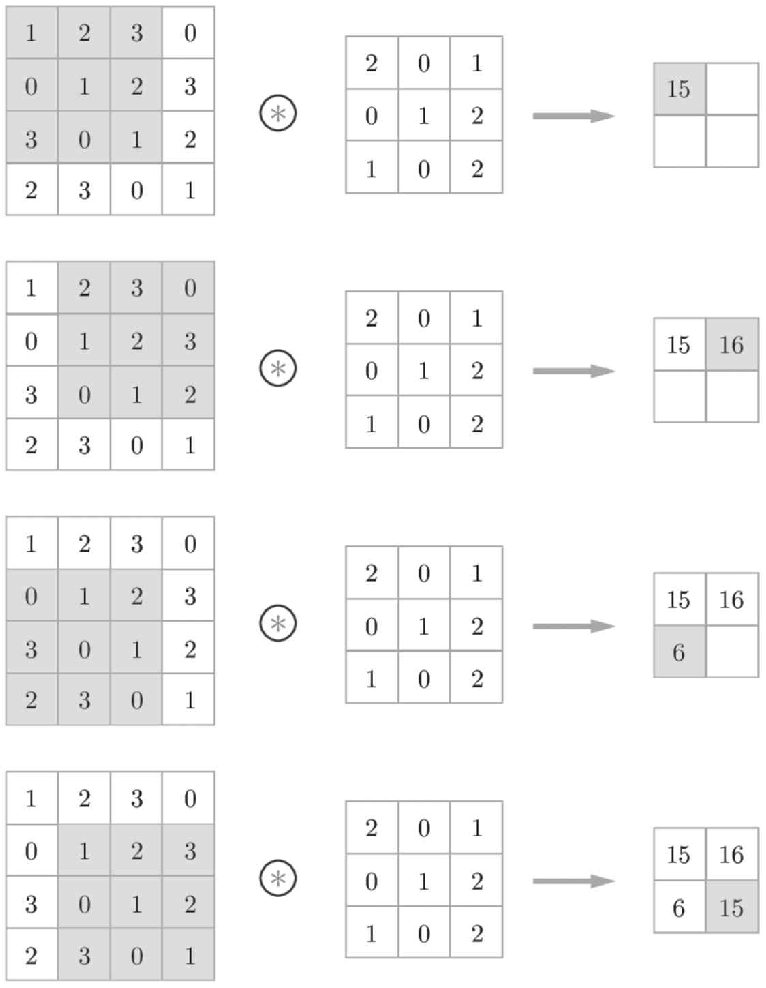
\includegraphics[width=1\columnwidth]{../Figure/Figure_3.pdf}
    \hlinefill
    \label{Fig.3}
\end{figure}
완전연결신경망에는 가중치 매개변수와 편향이 존재하는데, CNN에서는 필터 매개변수가 가중치에 해당한다. CNN에도 편향이 존재한다. 편향은 필터를 적용한 후 데이터에 더해진다. 편향은 항상 하나(1*1)만 존재한다. 하나의 값을 모든 원소에 더한다.
\begin{figure}[h!]
    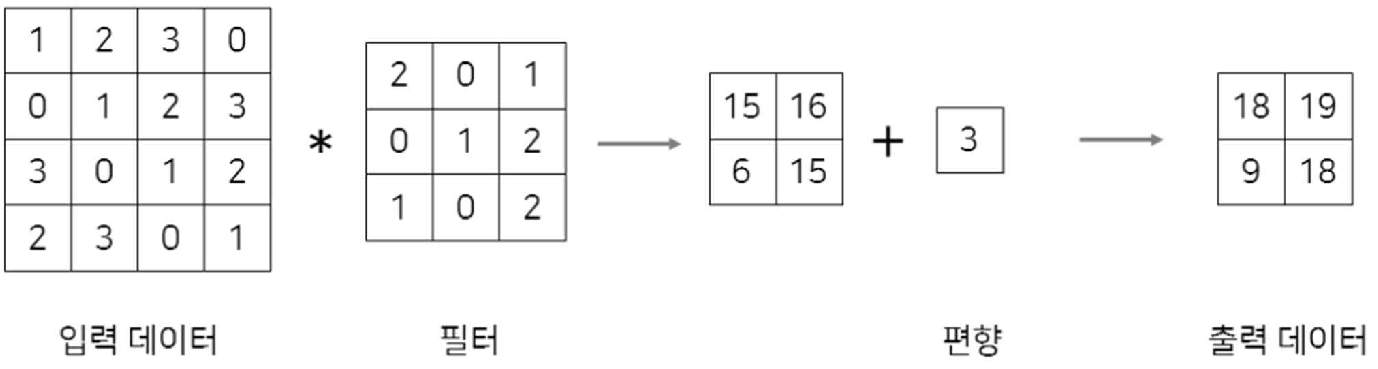
\includegraphics[width=1\columnwidth]{../Figure/Figure_4.pdf}
    \label{Fig.4}
\end{figure} 

\subsubsection{패딩}
합성곱 연산을 수행하기 전에 입력 데이터 주변을 특정 값으로 채우기도 한다. 이러한 작업을 패딩이라고 하며, 합성곱 연산에서 자주 이용하는 기법이다.
\begin{figure}[h!]
    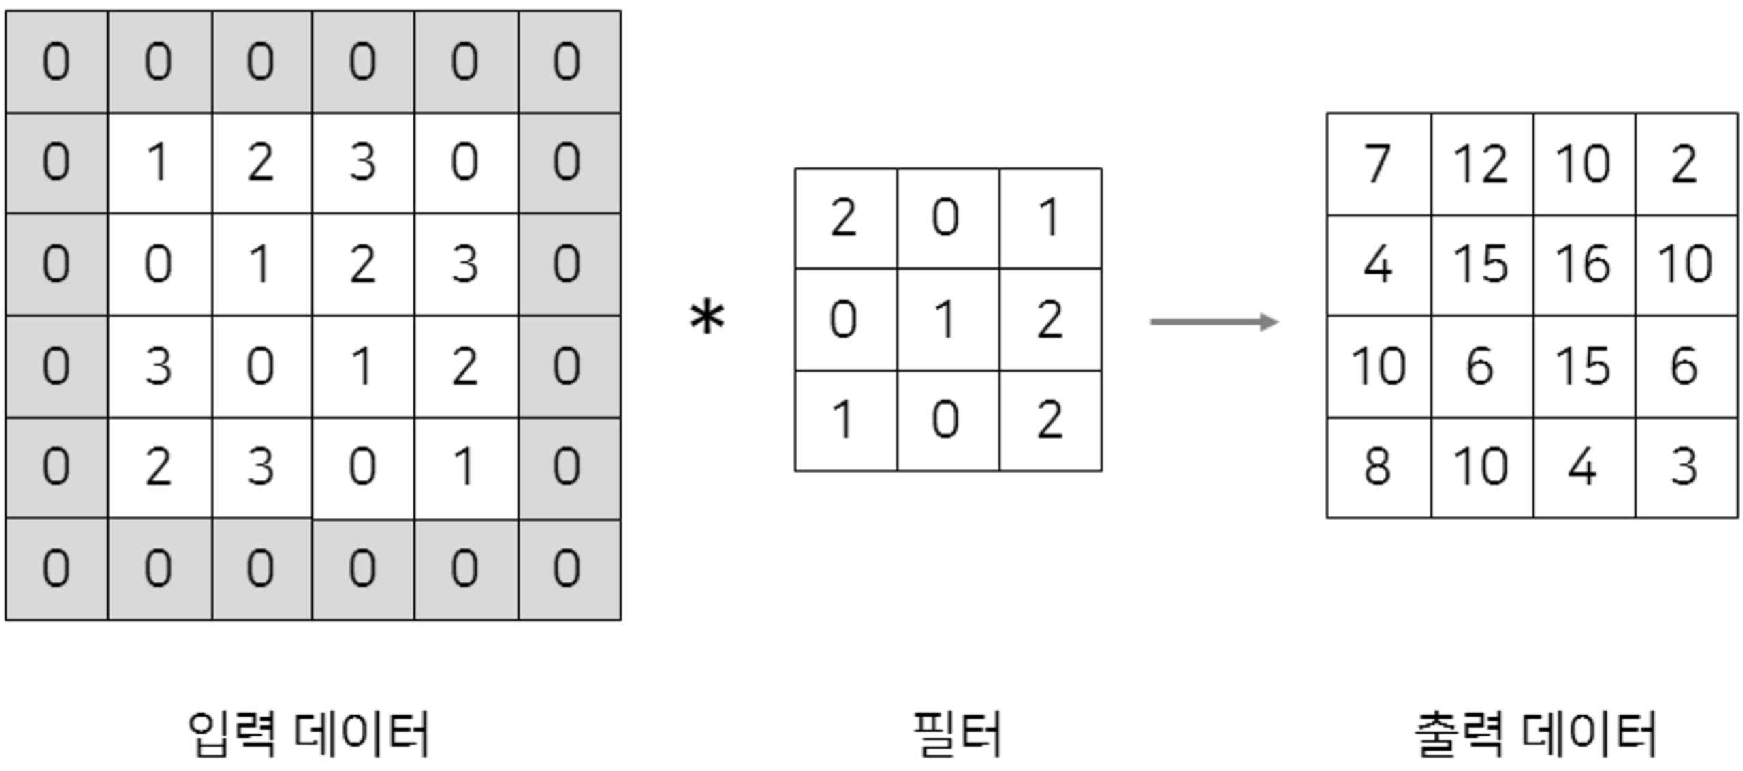
\includegraphics[width=1\columnwidth]{../Figure/Figure_5.pdf}
    \label{Fig.5}
\end{figure}  

\subsubsection{스트라이드}
\subsubsection{3차원 데이터의 합성곱 연산}
\subsubsection{블록으로 생각하기}
\subsubsection{배치처리}
\subsection{풀링계층}
\subsubsection{풀링계층의 특징}



$$ OH = \dfrac{H+2P-FH}{S} + 1 \\

$$ OW = \dfrac{W+2P-FW}{S} + 1 \\


\end{document}
